\subsection{Experimental Setup}
\label{sec:setup}

\subsubsection{System used}

We employ a server equipped with two Intel Xeon Gold 6226R processors, each featuring $16$ cores running at a clock speed of $2.90$ GHz. Each core is equipped with a $1$ MB L1 cache, a $16$ MB L2 cache, and a $22$ MB shared L3 cache. The system is configured with $376$ GB RAM and set up with CentOS Stream 8.


\subsubsection{Configuration}

We use 32-bit integers for vertex ids and 32-bit float for edge weights but use 64-bit floats for computations and hashtable values. We utilize $64$ threads to match the number of cores available on the system (unless specified otherwise). For compilation, we use GCC 8.5 and OpenMP 4.5.

%% From LP SRS
We use 32-bit integers for vertex ids and 32-bit float for edge weights but use 64-bit floats for computations and hashtable values. We utilize $64$ threads to match the number of cores available on the system.


\subsubsection{Dataset}

The graphs used in our experiments are given in Table \ref{tab:dataset}. These are sourced from the SuiteSparse Matrix Collection \cite{suite19}. In the graphs, number of vertices vary from $3.07$ to $214$ million, and number of edges vary from $25.4$ million to $3.80$ billion. We ensure edges to be undirected and weighted with a default of $1$.

%% From LP SRS
For the experiments, we use $13$ graphs from the SuiteSparse Matrix Collection\ignore{\cite{suite19}}. In the graphs, number of vertices vary from $3.07$ to $214$ million, and number of edges vary from $25.4$ million to $3.80$ billion. We ensure edges to be undirected and weighted with a default of $1$. For each graph, we generate uniformly random batch of edge deletions of size $10^{-7} |E|$ to $0.1 |E|$. For each batch size, we generate five random batch updates for averaging.

\begin{table}[hbtp]
  \centering
  \caption{List of $13$ graphs obtained SuiteSparse Matrix Collection \cite{suite19} (directed graphs are marked with $*$). Here, $|V|$ is the number of vertices, $|E|$ is the number of edges (after adding reverse edges), $D_{avg}$ is the average degree, and $|\Gamma|$ is the number of communities obtained with \textit{GVE-Leiden}.\ignore{In the table, B refers to a billion, M refers to a million and K refers a thousand.}}
  \label{tab:dataset}
  \begin{tabular}{|c||c|c|c|c|}
    \toprule
    \textbf{Graph} &
    \textbf{\textbf{$|V|$}} &
    \textbf{\textbf{$|E|$}} &
    \textbf{\textbf{$D_{avg}$}} &
    \textbf{\textbf{$|\Gamma|$}} \\
    % \textbf{$1 - \Gamma_G$} \\
    \midrule
    \multicolumn{5}{|c|}{\textbf{Web Graphs (LAW)}} \\ \hline
    indochina-2004$^*$ & 7.41M & 341M & 41.0 & 5.00K \\ \hline  % & \num{4.7e-4} & 2.9 GB
    uk-2002$^*$ & 18.5M & 567M & 16.1 & 43.1K \\ \hline  % & \num{9.6e-5} & 16 GB
    arabic-2005$^*$ & 22.7M & 1.21B & 28.2 & 3.80K \\ \hline  % & \num{5.5e-4} & 11 GB
    uk-2005$^*$ & 39.5M & 1.73B & 23.7 & 21.2K \\ \hline  % & \num{9.6e-5} & 16 GB
    webbase-2001$^*$ & 118M & 1.89B & 8.6 & 2.77M \\ \hline  % & \num{7.3e-7} & 18 GB
    it-2004$^*$ & 41.3M & 2.19B & 27.9 & 5.24K \\ \hline  % & \num{3.8e-4} & 19 GB
    sk-2005$^*$ & 50.6M & 3.80B & 38.5 & 3.75K \\ \hline  % & \num{5.8e-4} & 33 GB
    \multicolumn{5}{|c|}{\textbf{Social Networks (SNAP)}} \\ \hline
    com-LiveJournal & 4.00M & 69.4M & 17.4 & 2.33K \\ \hline  % & \num{7.9e-4} & 480 MB
    com-Orkut & 3.07M & 234M & 76.2 & 33 \\ \hline  % & \num{6.7e-2} & 1.7 GB
    \multicolumn{5}{|c|}{\textbf{Road Networks (DIMACS10)}} \\ \hline
    asia\_osm & 12.0M & 25.4M & 2.1 & 2.56K \\ \hline  % & \num{8.4e-4} & 200 MB
    europe\_osm & 50.9M & 108M & 2.1 & 3.61K \\ \hline  % & \num{6.6e-4} & 910 MB
    \multicolumn{5}{|c|}{\textbf{Protein k-mer Graphs (GenBank)}} \\ \hline
    kmer\_A2a & 171M & 361M & 2.1 & 19.4K \\ \hline  % & \num{9.4e-5} & 3.2 GB
    kmer\_V1r & 214M & 465M & 2.2 & 8.60K \\ \hline  % & \num{3.2e-4} & 4.2 GB
  \bottomrule
  \end{tabular}
\end{table}
% We convert directed graphs (marked with $*$) to undirected by duplicating edges in the reverse direction, and set the weight of each edge to $1$. and $F_{size}$ is size of the \textit{MatrixMarket} file

% \input{src/fig-leiden-compare}
% \input{src/fig-gve-compare}




\subsection{Comparing Performance of GVE-Leiden}

Upon each graph with edge deletions of batch size $B$ applied, we then predict the same number of edges $B$ using both JC and HP similarity scores. As mentioned in Section \ref{sec:approach}, we avoid high-degree first-order neighbors. For this, we adjust the degree threshold $D$ from $4$ to $32$ in multiples of $2$.

Figure X shows the average runtime of link prediction with degree threshold $D$ of $4$, $8$, $16$, and $32$. Increasing $D$ increases runtime by a small amount, due to increase second-degree neighbor exploration. Increasing/decreasing the batch size however does not have an effect on runtime, as the algorithm must continue to explore possible links with higher scores even if batch/prediction size $B$ edges have been added to the prediction list. Note that runtime for link prediction with JC/HP similarity scores is nearly identical. On a batch size of $0.1 |E|$, we compare the predicted links with the links in the original graphs (without edge deletions). We observe that HP-based link prediction with $D = 16$ obtains the highest average accuracy of $2.4\%$, while HP-based link prediction with $D = 4$ obtains the highest average precision of $6.4\%$. Given the vast set of potential predictions (${}_N C_2 - |E|$), achieving high accuracy and precision remains a challenge.

TODO.

\begin{figure*}[hbtp]
  \centering
  \subfigure[Runtime in seconds (logarithmic scale) for link prediction using the best similarity measure, with \textit{IHub} and \textit{LHub} approaches]{
    \label{fig:input-large--runtime}
    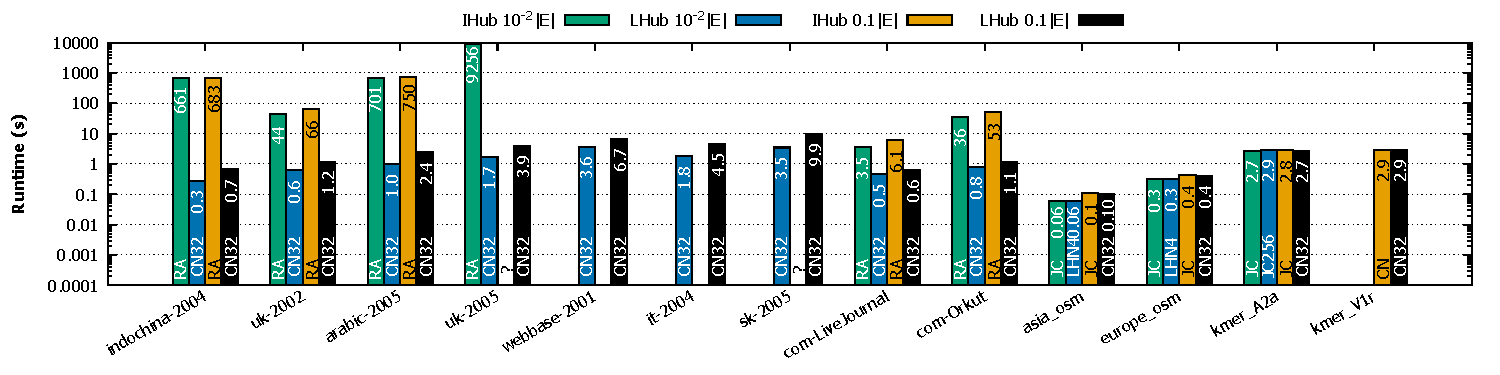
\includegraphics[width=0.98\linewidth]{out/input-large-runtime.pdf}
  }
  \subfigure[Speedup (logarithmic scale) for link prediction with the best similarity measure of \textit{LHub} approach, compared to \textit{IHub} approach]{
    \label{fig:input-large--speedup}
    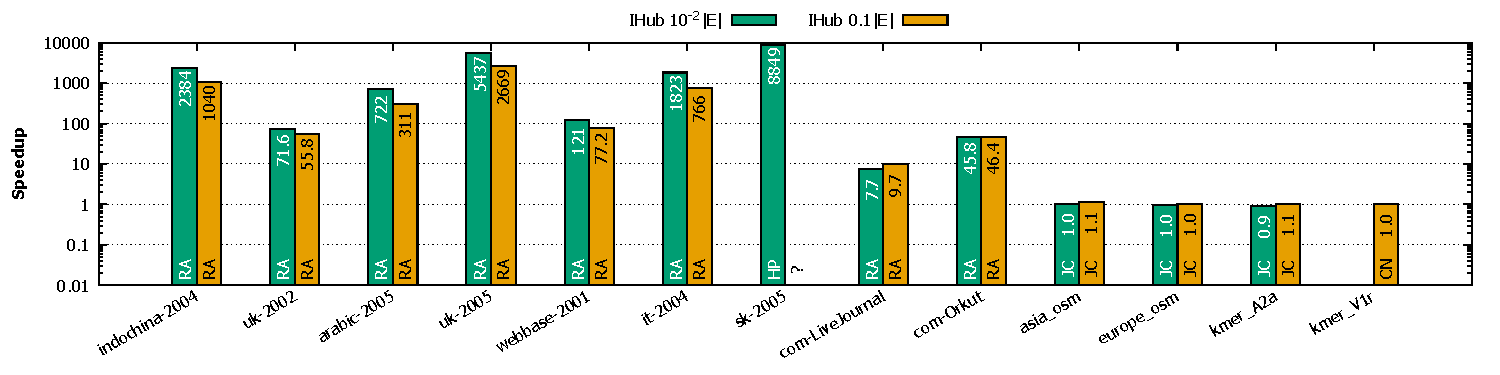
\includegraphics[width=0.98\linewidth]{out/input-large-speedup.pdf}
  }
  \subfigure[F1 score of predicted links (logarithmic scale), for link prediction using the best similarity measure, with \textit{IHub} and \textit{LHub} approaches]{
    \label{fig:input-large--f1score}
    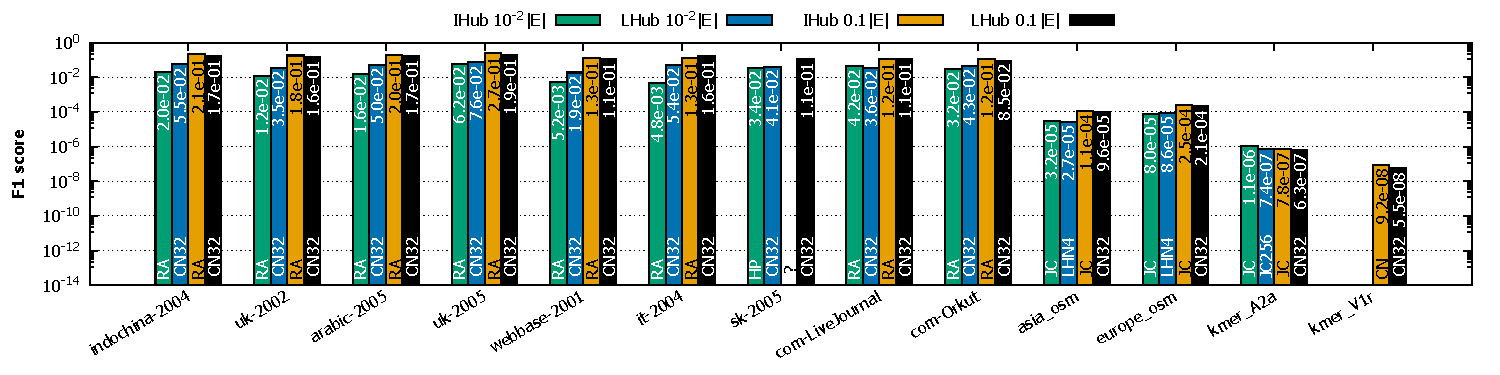
\includegraphics[width=0.98\linewidth]{out/input-large-f1score.pdf}
  } \\[-2ex]
  \caption{Runtime in seconds (log-scale), speedup (log-scale), and F1 score of predicted links (log-scale), for link prediction method using the best similarity measure, when attempting to predict $10^{-2}|E|$ to $0.1|E|$ unobserved edges $E^U$, for each graph in the dataset. For each similarity measure outlined in Section \ref{sec:metrics}, we attempt only the best hub limit $L_H$ parameter setting obtained in Section \ref{sec:select-limit} (for the \textit{LHub} approach), and then select the best among them, considering both the F1 score and runtime. Note that the numerical suffix added to the acronym of each link prediction method, with the \textit{LHub} approach, indicates the hub limit $L_H$ parameter setting.}
  \label{fig:input-large}
\end{figure*}

\begin{figure}[hbtp]
  \centering
  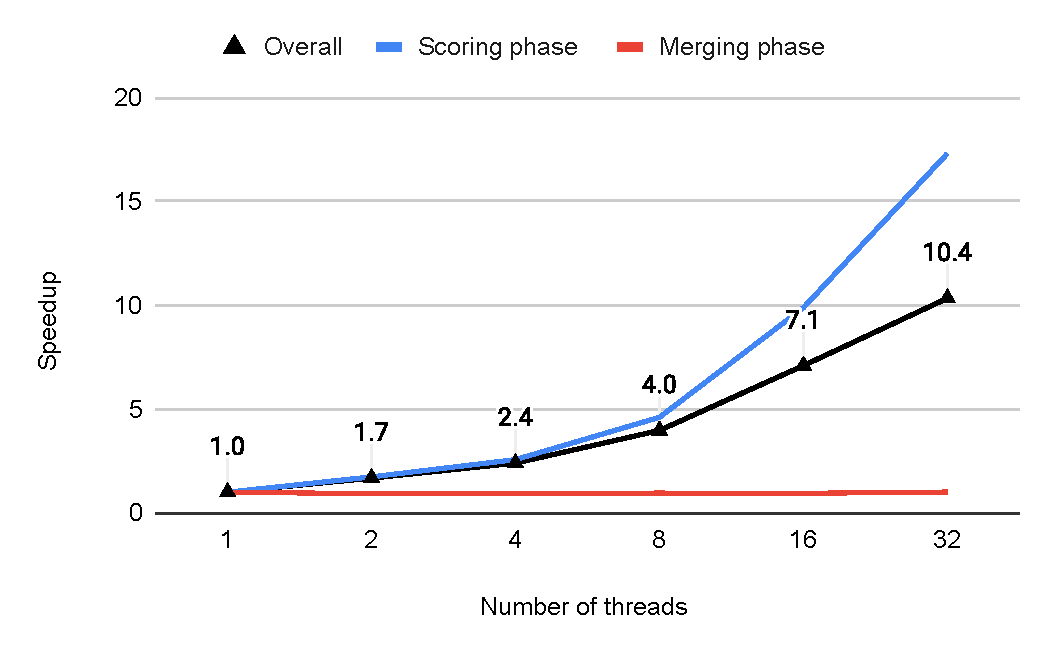
\includegraphics[width=0.98\linewidth]{out/strong-scaling-speedup.pdf} \\[-2ex]
  \caption{Overall speedup of our approach of \textit{Disregarding Large Hubs (DLH)} for link prediction, and its phases (obtaining edges with top-k scores per thread, and merging scores from each thread into a common scoreboard), with $10^{-2}|E|$ unobserved edges, with increasing number of threads (in multiples of 2). Increasing the number of threads causes work in the merging phase to increase,\ignore{thus} leading to a poor speedup.}
  \label{fig:strong-scaling}
\end{figure}





\subsection{Analyzing Performance of GVE-Leiden}

TODO.




\subsection{Strong Scaling of our Optimized Neighbor-based Link Prediction Methods}

Finally, we assess the strong scaling performance of our optimized neighbor-based link prediction methods. In this analysis, we vary the number of thread from $1$ to $32$ in multiples of $2$ for each input graph, and measure the average time taken to predict $10^{-2}|E|$ links by Hub Promoted (HP), Leicht-Holme-Nerman (LHN), Adamic-Adar Coefficient (AA), and Resource Allocation (RA) based link prediction methods with the \textit{MAX\_MEDIATOR\_DEGREE} parameter set to $4$. The results are shown in Figure \ref{fig:strong-scaling}. It not only illustrates the overall scaling performance, but the also scaling of the two phases of each link prediction method, i.e., identifying edges with top-k scores in each thread (scoring phase), and combining the scores obtained by each thread to obtain the global top-k edges (merging phase). With $32$ threads, our optimized link prediction methods achieve an overall speedup of $7.2\times$ (with respect to sequential execution), indicating a performance increase of $1.5\times$ for every doubling of threads. The scalability is limited, as the cost of the merging phase increases with an increase in the number of threads. In fact, at $32$ threads, the merging phase obtains a speedup of $0.7\times$ (yes it is less than $1$\ignore{, as its runtime increases}), while the scoring phase achieves a speedup of $18.5\times$.

\begin{figure*}[hbtp]
  \centering
  \subfigure[Runtime]{
    \label{fig:input-small--runtime}
    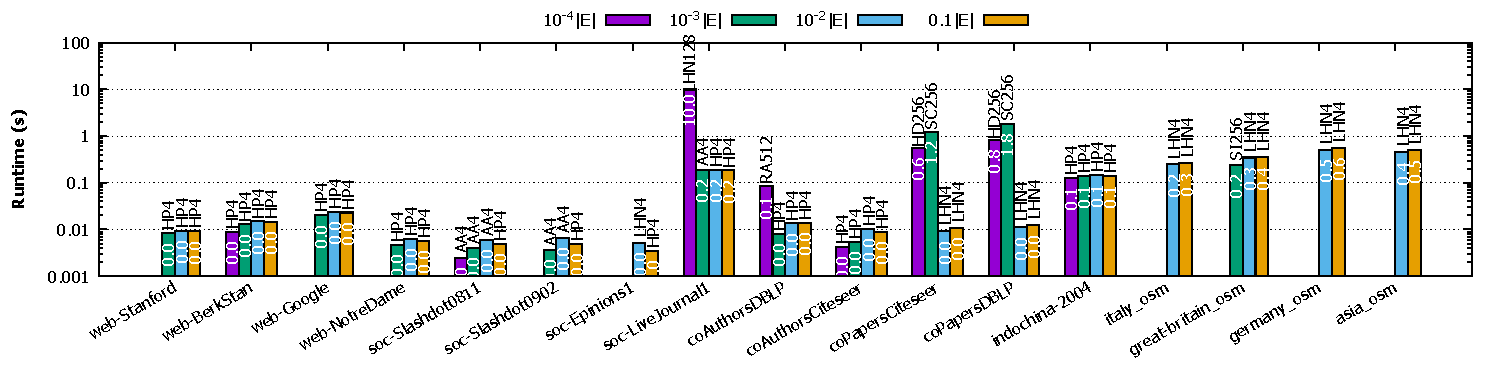
\includegraphics[width=0.98\linewidth]{out/input-small-runtime.pdf}
  }
  \subfigure[Precision]{
    \label{fig:input-small--precision}
    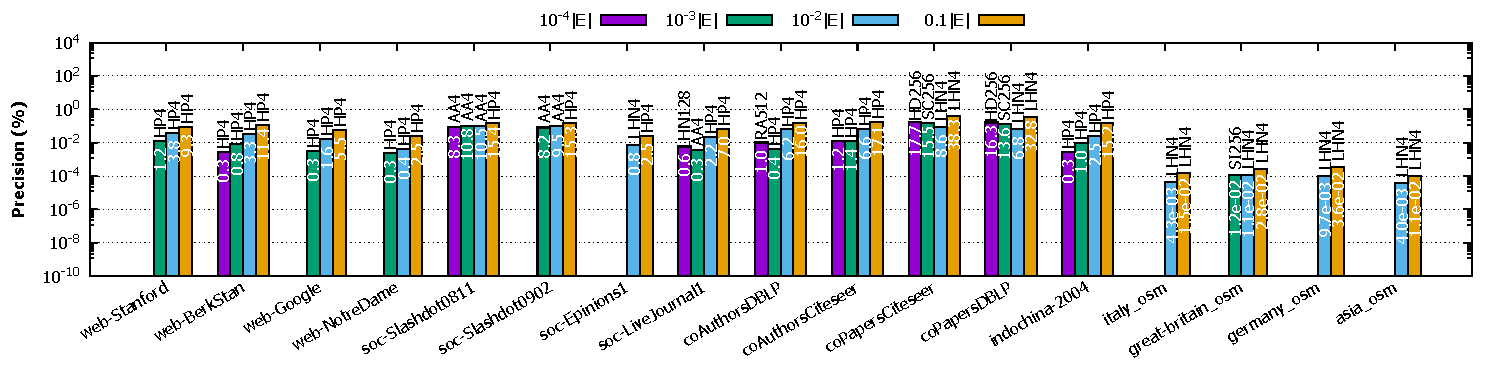
\includegraphics[width=0.98\linewidth]{out/input-small-precision.pdf}
  } \\[0ex]
  \caption{TODO. Input small.}
  \label{fig:input-small}
\end{figure*}

